% TU Delft beamer template
% Author: Erwin Walraven (initial version was created by Maarten Abbink)
% Delft Universiy of Technology

\documentclass{beamer}
%\usepackage[english]{babel}
%\usepackage{calc}
%\usepackage[absolute,overlay]{textpos}
%\usepackage{graphicx}
%\usepackage{subfig}
%\usepackage{amsmath}
%\usepackage{amsfonts}
%\usepackage{amsthm}
%\usepackage{mathtools}
%\usepackage{comment}
%\usepackage{MnSymbol,wasysym}

\usepackage{multirow}
\usepackage{makecell}
\usepackage{tikzsymbols}
\setbeamertemplate{caption}[numbered]



\setbeamertemplate{navigation symbols}{} % remove navigation symbols
\mode<presentation>{\usetheme{tud}}

% BIB SETTINGS
% \usepackage[backend=bibtex,firstinits=true,maxnames=30,maxcitenames=20,url=false,style=authoryear]{biblatex}
% \bibliography{bibfile}
% \setlength\bibitemsep{0.3cm} % space between entries in the reference list
% \renewcommand{\bibfont}{\normalfont\scriptsize}
% \setbeamerfont{footnote}{size=\tiny}
% \renewcommand{\cite}[1]{\footnote<.->[frame]{\fullcite{#1}}}


\title[]{Research Progress}
\institute[]{Delft University of Technology, The Netherlands}
\author{Jie Liu}
%\date{}

\begin{document}
{
\setbeamertemplate{footline}{\usebeamertemplate*{minimal footline}}
\frame{\titlepage}
}


\begin{frame}
\frametitle{Problem statement}
\vspace{-8em}
\begin{block}{Equation to be solved}
\scriptsize
\begin{equation}
 \nabla \cdot (T_1 \nabla u) + T_2 \frac{\partial{u}}{\partial{x}} + T_3 \frac{\partial{u}}{\partial{y}} + T_4 u = f,\qquad (x,y) \in \Omega = [0,\,1] \times [0,\,1],
 \label{problem_to_be_investigated}
\end{equation}
where, $T_1$, $T_2$, $T_3$ and $T_4$ are coefficient functions\footnote{$T_2$ and $T_3$ have not been included practically in the code yet.}.
\end{block}
\end{frame}


\begin{frame}{FEM Status}
\vspace{-3em}
The status of the application of FEM methods on various second order differential problems (Poisson, diffusion and Helmholtz) is shown in Table~\ref{table_status_fem_application}.

\begin{table}[!ht]
\scriptsize
\begin{tabular}{l | l | c }
\multicolumn{2}{c|}{} & \makecell{Problems with real/complex-\\valued solution} \\ \hline
\multirow{2}{*}{1D} & Standard FEM ($P_p$) & $\Smiley$ (working well) \\ \cline{2-3}
 & Mixed FEM ($P_p/P_{p-1}^{\rm disc}$) & $\Smiley$ \\ \hline
\multirow{3}{*}{2D} & Standard FEM ($P_p$) & $\Smiley$ \\ \cline{2-3}
 & Mixed FEM ($RT_p/P_{p}^{\rm disc}$) & $\Smiley$ \\ \cline{2-3}
 & Mixed FEM ($BDM_p/Q_{p-1}^{\rm disc}$) & $\Neutrey$\footnote{Only working for only Dirichlet boundary conditions, not working when Neumann boundary conditions are considered.} 
\end{tabular}
\caption{Status of application of FEM methods on different problems}
\label{table_status_fem_application}
\end{table}
\end{frame}


\begin{frame}{Future work}
\vspace{-10em}
\begin{itemize}
 \item To consider $T_2$ and $T_3$ parts in Eq.~(\ref{problem_to_be_investigated}).
 \item To implement $BDM_p/Q_{p-1}^{\rm disc}$ elements for Neumann boundary conditions, and then determine which elements to use to obtain $\alpha_{\rm R}$ and $\beta_{\rm R}$ for the mixed FEM.
\end{itemize}

\end{frame}

%\begin{frame}{Pictures}
%\begin{figure}
%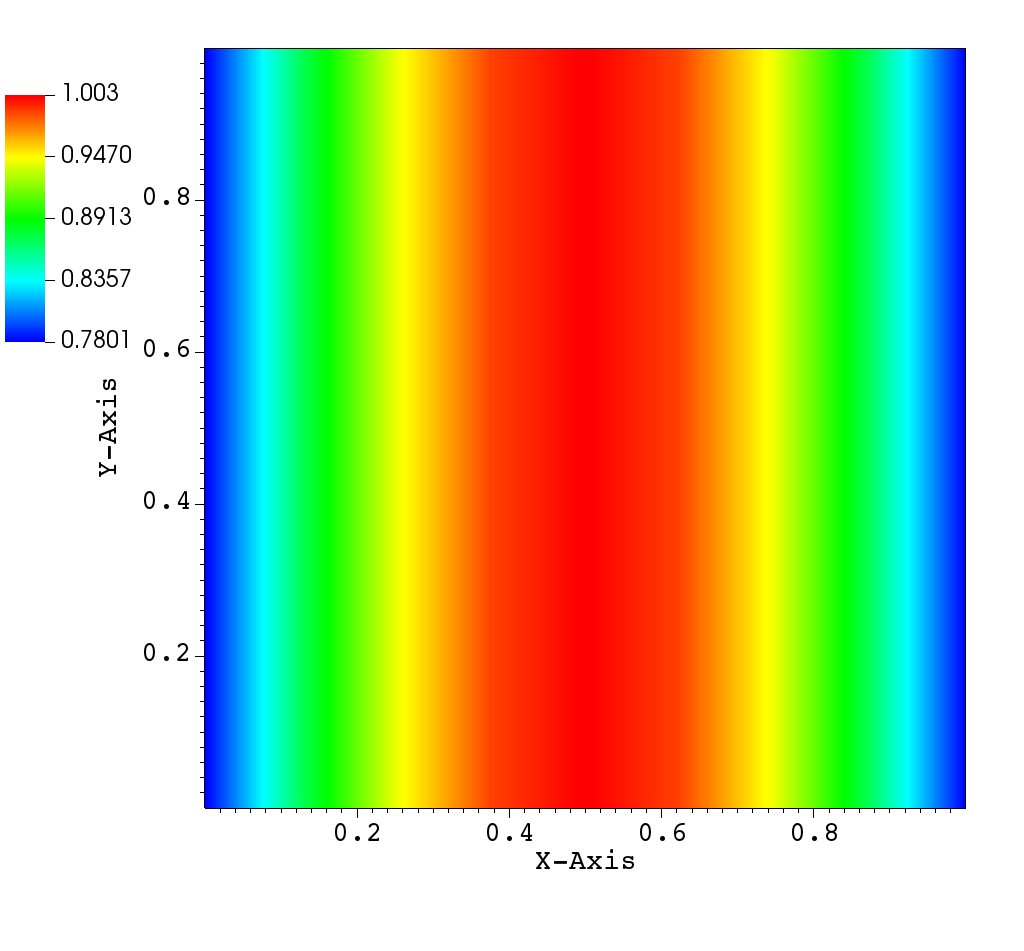
\includegraphics[width=0.5\linewidth]{Shape_TwoD_u_exp_xm0p5squared_pressure.png}
%\caption{lion!!}
%\end{figure}
%Thank you.
%\end{frame}

\end{document}
